\chapter{Callback \& Signals und Slots - Interaktion}

\section{Reaktive Systeme}

Reaktive Systeme (reactive systems) reagieren auf (oft externe) Ereignisse wie digitale Inputs, die Erreichung von analogen Schwellenwerten, Timer, Buttonclicks oder ähnliches in GUI, etc. Dabei bestehen häufig auch Echtzeitanforderung an das System. Embedded Systems sind häufig auch reaktive Systeme. 
Ereignisse sind per Definition asynchron, d.h. sie treten zu einem beliebigen Zeitpunkt ein, während ein "normales" Programm immer synchron (zuerst das, dann das, dann …) ist. 

\subsection{Pooling}
Ereignisse können von synchronen Programmen durch Polling verarbeitet werden, d.h. das 
Programm fragt periodisch oder dauernd ab, ob irgendein Ereignis eingetreten ist. Polling ist sehr einfach zu implementieren. 
Dabei entstehen jedoch üblicherweise sehr viele Leerabfragen, d.h. bei vielen Abfragen ist nichts eingetreten, was eine unnötige Prozessorbelastung bewirkt. Sie können durch periodische Abfragen (Kopplung an Timer) reduziert aber nicht vermieden werden.
Die maximale Reaktionszeit wird durch die Abfrageperiode und die Anzahl Abfragen (Stichwort: Looptime bei SPS) definiert. 

\subsection{C Callbacks}
Callbacks stellen bidirektionale Verbindungen von Modulen mit C dar. 

\textbf{Beispiel einer bidirektionalen Verbindung zwischen A und B} \\
 Dabei kennt Klasse A, B UND Klasse B kennt ebenfalls die Funktion von Klasse A.
C-File von A: \\
void aInit(void) \\ \{
	bRegisterFoo(\&aFooY);  \textbackslash*Eine Funktion von B wird in A aufgerufen. Der Parameter der Funktion ist eine Funktion der Klasse A. /* 
\}\\
void aFooY(void) \\ \{ 
	printf("aFooY called\textbackslash n");
\}

C-File von B: \\
static void (*regFct)(void); \% Funktionspointer \\
void bFooX(void) \\
\{ 
	if (0 != regFct)\\
	regFct();
\}\\
void bRegisterFoo(void (*fct)(void))\\
\{
	regFct = fct; \textbackslash* Die von der Klasse A aufgerufene Funktion bRegisterFoo hat als Parameter eine Funktion aus der Klasse A, welche dem Funktionspointer regFct zugewiesen wird und wieder auf die Funktion aFooY in der Klasse A zeigt. /*
\}



\textbf{Beispiel einer unidirektionalen Verbindung zwischen Klasse A und B} \\
Dabei hat die Klasse A eine Verbindung zu Klasse B, aber nicht umgekehrt. 

Das File der Kasse A sieht folgendermassen aus: \\
\textbf{\#include "B.h"  \% Das Header File von B wird eingefügt}
class A \\
{ public: \\
	\textbf{A() { b.foo();	}  \% Verknüpfung mit B}\\
	void fooY() {} \\
	private: \\
	\textbf{B b; \% Ein Objekt der Klasse B kann somit in A aufgerufen werden} \\
};

\textbf{Bidirektionale Verbindung von Klassen} \\
Klasse A kennt Klasse B UND Klasse B kennt Klasse A -> Das funktioniert so nicht, da es sich um ein circular include handelt. Eine Ausnahme stellt ein Class Forwarding dar. \\
\begin{figure}[ht]
	\adjustbox{width=9cm}{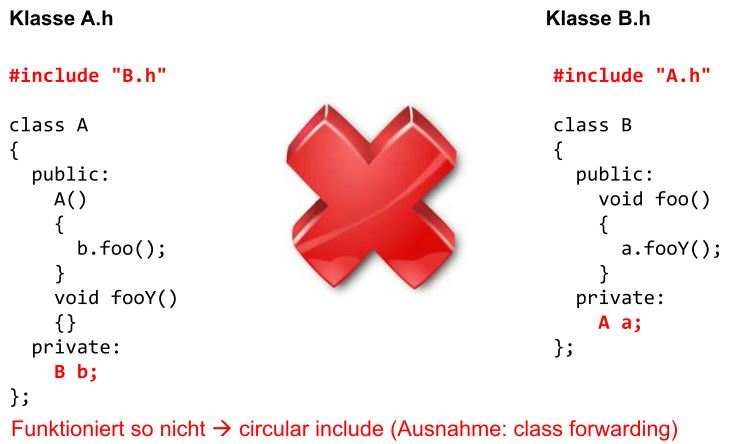
\includegraphics{Figures/bidirektional}}
	\caption[]{Keine gültige Bidirektionale Verbindungen von A und B}
\end{figure}

Die nachfolgenden Versionen einer bidirektionalen Verbindung: \\
V1:Klasse A kennt Klasse B UND Klasse B kennt Objekt von Klasse A
Funktioniert, da in Header-File B.h nur Pointer auf A, der Rest ist im B.cpp File. Unschön: B muss immer noch A kennen (class forwarding erforderlich). Besser: A sollte unabhängig von B sein

V2:Klasse A kennt Klasse B UND Klasse B kennt Objekt von Klasse C, Klasse A ist eine Klasse C. Bessere Variante als V1: B kennt nicht mehr A direkt

V3:Klasse A kennt Klasse B UND Klasse B kennt Objekt von Klasse C, Klasse A ist eine Klasse C. Besser Variante als V2: der Funktionspointer wird weggelassen, da überflüssig

\begin{figure}[ht]
\adjustbox{width=12cm}{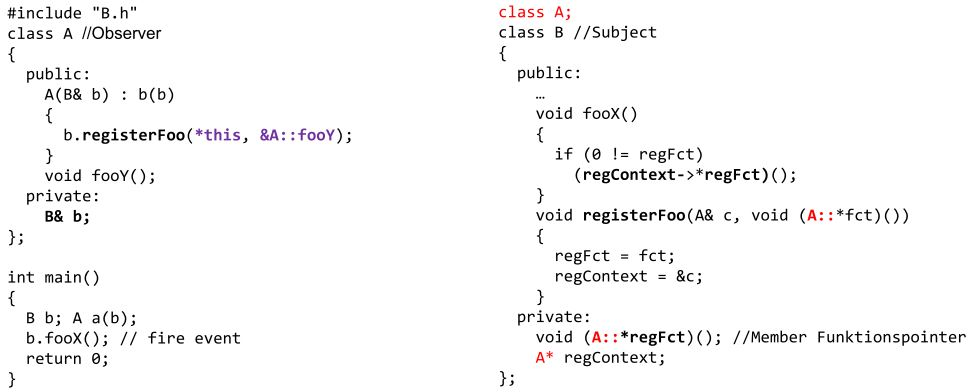
\includegraphics{Figures/bidirektionalv1}}
\adjustbox{width=12cm}{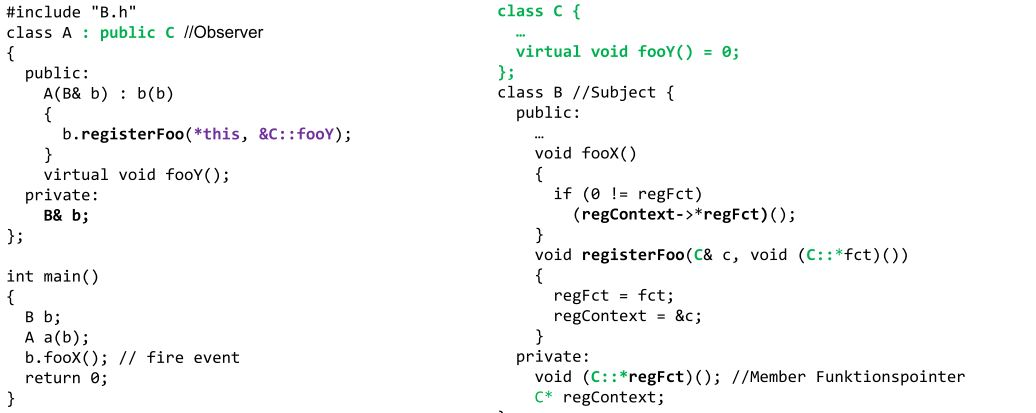
\includegraphics{Figures/bidirektionalv2}}
\adjustbox{width=12cm}{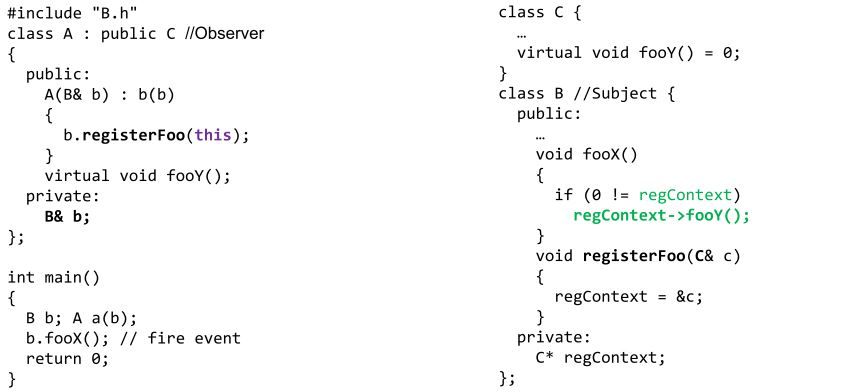
\includegraphics{Figures/bidirektionalv3}}
\caption[]{Bidirektionale Verbindungen: V1-V3}
\end{figure}

Abstraktere C++ Umsetzungen folgen im Modul OOAD: Observer Pattern. 
Die kennengelernten Callback und Observer Methoden können für native C++ verwendet werden. In Qt können Signal/Slots verwendet werden.

\section{Qt Signals and Slots: Qt Interaktion zwischen QObjects}

Qt verwendet anstatt Callbacks ein Signal-Slot Prinzip. Analogie zu Callbacks: Das zu informierende Objekt (Observer) hat einen slot, Das informierende Objekte (Subject) hat ein signal, die Registrierung erfolgt über eine connect Funktion. 

Es wird der Funktionspointer von C++-Member verwendet. Signals und Slots werden mit dem QObject::connect() verbunden. \\ 
Form: connect(SenderObj* (=Subject), SenderMethode* (signal1), EmpfängerObj* (= Observer), EmpfängerMethode* (slot2)) \\
Bsp.: connect(\&b, \&B::fooX, \&a, \&A::fooY);

Beispiel: 
\begin{figure}[ht]
	\centering
	\adjustbox{width=0.9\textwidth}{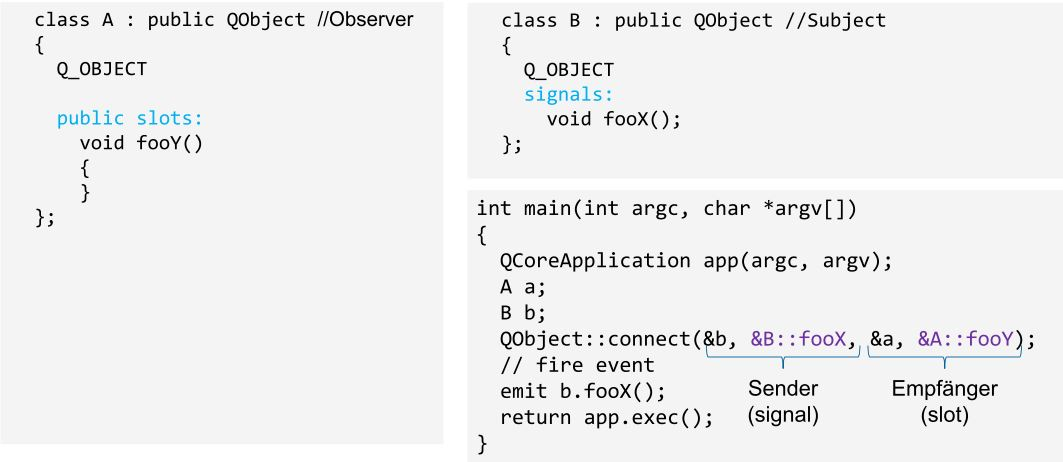
\includegraphics{Figures/bspsignal}}
	\caption[]{Beispiel Signal \& Slots}
\end{figure}

%\begin{figure}[ht]
%	\centering
%	\adjustbox{width=0.9\textwidth}{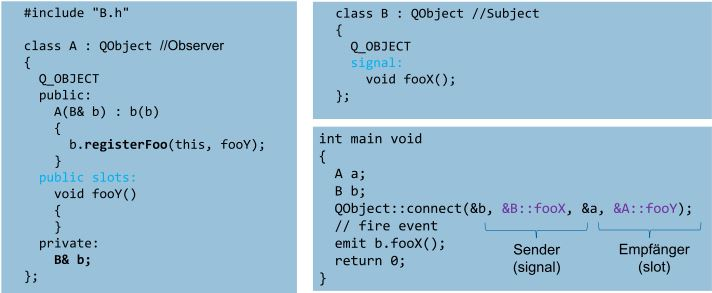
\includegraphics{Figures/bspsigslot}}
%	\caption[]{Beispiel Signal \& Slots}
%\end{figure}

\subsection{Signals - Signal-Memberfunktion}
Signals werden nur deklariert und nicht implementiert. Es werden keine Zugriffsrechte wie private public oder protect verwendet. Der Rückgabetyp ist immer void. Ein Signalaufruf erfolgt mit \textbf{emit method(value)}. Die C++ Definition erfolgt mit \textbf{\#define signals public}. Ein Signal kann mit mehreren Slots oder anderen Signalen verbunden werden. Mehrere Signal können mit demselben Slot verbunden werden. Es kann einen Übergabeparameter haben.

\subsection{Slots}
Slots sind immer public (by default). Für private slots muss das Keyword slots weggelassen werden. Die C++ Definition lautet \textbf{\#define slots}. Slots können einen Übergabeparameter haben. 

\subsection{Signals \& Slots: Connect}

Der Parameter Typ und Anzahl muss stimmen
Signal: Slot:
void clicked() -> void onClicked()
void indexChanged(int idx) -> void onIndexChanged(int idx)


\textbf{Ab Qt5 - mit Funktionspointer} \\
connect(senderObj, \&SenderClass::senderMethod \\
revObj, \&RevClass:revMethod); \\
+ weniger Klammern  \\
+ keine Datentypen für Parameter; aber Compiler meldet Fehler

\textbf{Alte Notation} \\
connect(button, SIGNAL(clicked()) \\
count, SLOT(incValue())); \\
Keine Compilerfehlermeldungen, falls falsch -> wird zur Laufzeit geprüft

\textbf{Globale Funktionen als Slots (ab Qt5)} \\
void printValue(int x) \\
\{ 	std::count << "Value=" << x << std::endl;\} \\
connect(button, \&QPushButton::clicked, \&printValue); 


\textbf{Überladene Methoden} \\
void QLabel::setNum(int num) \\
void QLabel::setNum(double num) \\
connect(…, static\_cast<void (QLabel::*)(int)>(\&QLabel::setNum), …, …);

\begin{figure}[ht]
	\centering
	\adjustbox{width=0.7\textwidth}{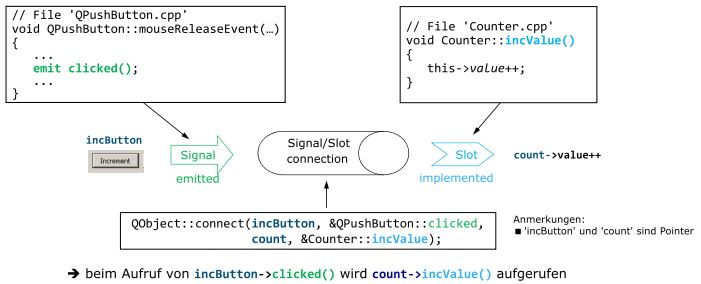
\includegraphics{Figures/sigausframework}}
	\caption[]{Beispiel mit Signal aus Framework}
\end{figure}

\begin{figure}[ht]
	\centering
	\adjustbox{width=0.7\textwidth}{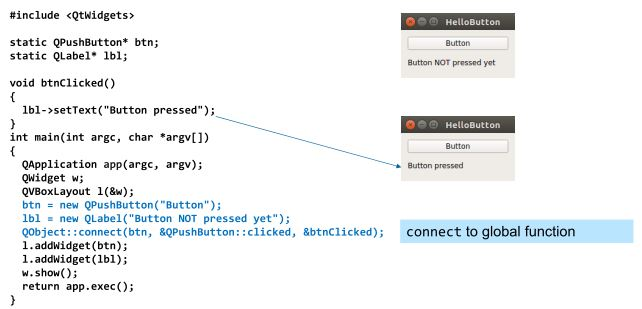
\includegraphics{Figures/hellobutton}}
	\caption[]{"Hello Button" - GUI Programm}
\end{figure}

\begin{figure}[ht]
	\centering
	\adjustbox{width=9cm}{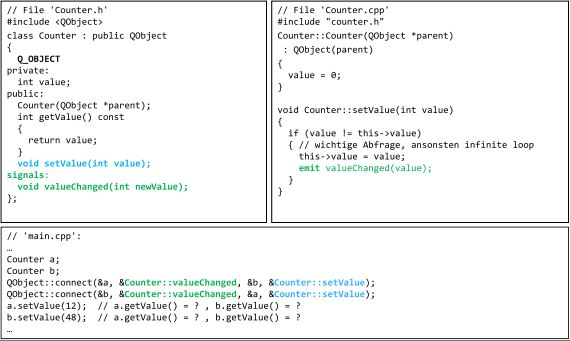
\includegraphics{Figures/selfconnect}}
	\caption[]{Counter Beispiel: Connect mit sich selbst}
\end{figure}


